\chapter{Phenotypic and Molecular Characterization of \emph{rpoS} from \e{Pseudomonas syringae} Lz4W}

\section{Introduction}
\label{chap6:intro} In previous Chapters it was shown that
\lzsig{} harbors an amber mutation in its reading-frame which
could potentially produce a truncated, yet functional RpoS, at
least as far as the induction of \bact{Ec} promoters is concerned.
It were demonstrated in several studies that \emph{rpoS}, in a
wide range of bacterial species, is prone to mutation.
Interestingly, it was also observed that the stationary phase
cultures of \bact{Ec} are easily taken over by mutants that have
selective advantage over the ancestral
population~\citep{Zambrano1993}. These mutants, aptly termed as
``GASP'' (\emph{G}rowth \emph{A}dvantage in \emph{S}tationary
\emph{P}hase), are able to grow when the ancestral population can
not. These GASP mutants, apparently, are able to reinitiate growth
by scavenging nutrients released by dying
cells~\citep{Zinser1999}. In fact, multiple rounds of mutants
arise to take over the ancestral population during prolonged
starvation~\citep{Finkel1999}. Although, GASP mutations are of
different kinds, some involved in amino acid
catabolism~\citep{Zinser1999}, some are in transcription factor
such as \emph{lrp}~\citep{Zinser2000}, the striking fact is that
the first round of mutations that take over the culture, are more
often than not located in \emph{rpoS}~\citep{Vulic2001}.

Given, that \emph{rpoS} controls the general stress response in
\bact{Ec} and related bacteria, and influence the survivality at
stationary phase, GASP mutants creates a paradox in the field.
This apparent paradox was addressed in a recent study where it was
shown that \emph{rpoS} mutation has a selective advantage during
slow growth in chemostat culture of \bact{Ec}~\citep{Mcrobb2002}.
It was proposed that \emph{rpoS} mutation causes an upregulation
of \emph{rpoD} controlled genes, which confers a selective
advantage through increase in outer membrane permeability and
increased nutrient scavenging under low nutrient
conditions~\citep{Mcrobb2002}. Interestingly, in conditions of
dual stress, like low pH and carbon starvation, majority of the
\emph{rpoS} GASP mutations are not null but attenuated
\emph{rpoS}, containing amber. This observation led the authors to
conclude that amber mutation in \emph{rpoS} is a mechanism to
reduce, at the same time maintaining enough \emph{rpoS} activity
to cope with the stress condition, such as low pH.

Low temperature is one of the known stress conditions that
increases RpoS level in \bact{Ec}. In \bact{Ec}, RpoS protein is
unstable and is present only in small amounts during exponential
growth at 37\dg{}~\citep{Lange1994}. The level of RpoS, however,
increases during exponential growth at low temperature (20\dg{}),
mediated by a 87 nucleotide long RNA, DsrA~\citep{Sledjeski1996}.
DsrA functions through an \emph{anti-anti-sense} mechanism that
disrupts intramolecular basepairing in \emph{rpoS} mRNA,
facilitating \emph{rpoS} translation at low
temperature~\citep{Majdalani1998,Lease1998,Lease2000}.

Upregulation of the \emph{rpoS} was  reflected in upregulation of
several \emph{rpoS}-controlled promoters at low temperature,
measured using \emph{lacZ}
fusions~\citep{Sledjeski1996,Rajkumari2001}. The role of
\emph{rpoS} in growth at low temperature, however, remains
elusive. \emph{rpoS} mutant, grew as fast as the wild-type cells
at low temperature~\citep{Sledjeski1996}.

Contrary to its role during growth at low temperature, the role of
\emph{rpoS} in other stress conditions are well defined. Two of
the several stress responses where \emph{rpoS} plays a crucial
role are, acid stress and oxidative stress. Although, the
mechanism is not clearly understood, \emph{rpoS}-dependent
acid-tolerance in \bact{Ec} and related bacteria is well
documented~\citep{Small1994,Cheville1996,Lee1995}. Acid
sensitivity of \emph{rpoS} mutants has been shown in a wide range
of bacterial species, including
\emph{Pseudomonas}~\citep{Jorgensen1999}.

The underlying mechanism, how cells cope with oxidative stress in
\emph{rpoS}-dependent manner is well understood in \bact{Ec}. The
bacterium is known to possess two catalases, HPI, encoded by
\emph{katG}, and HPII encoded by \emph{KatE}\@. HPI is a
hydroperoxidase, tetramer of \U{80,049}{Da} subunits, induced by
H\sub{2}O\sub{2} and associated with the plasma membrane in
\bact{Ec}~\citep{Schellhorn1995,Heimberger1988,Loewen1985}. The
induction of \emph{katG} by H\sub{2}O\sub{2} is mediated through
OxyR, which directly senses the oxidative stress and is activated
by conformational change upon oxidation occurring at a key
cysteine residue~\citep{Storz1990}. HPII hydroperoxidase, on the
otherhand, is a hexamer of \U{93,000}{Da} subunits and mainly
restricted to cytoplasm
\citep{Schellhorn1995,Heimberger1988,Loewen1985,Loewen1986,Loewen1984a}.
HPII level increases 10--20 folds during entry into stationary
phase but it is not induced by H\sub{2}O\sub{2}. \emph{katE}, the
gene encoding HPII was found to be controlled by \emph{rpoS}. In
fact, one of the first phenotypes identified for \emph{rpoS} was
severe catalase deficiency of \emph{rpoS} mutant, and \emph{rpoS}
was therefore, named as \emph{katF}~\citep{Loewen1984b}.

There is, however, contradictory reports about the role of
\emph{rpoS} in HPI expression. While an earlier report suggested a
\emph{rpoS}-dependent increase of \emph{katG} activity during
stationary phase~\citep{Ivanova1994}, a later report showed that
the increase of HPI level is not dependent on
\emph{rpoS}~\citep{Visick1997}. Moreover, in \emph{rpoS} mutant,
there was an increase in HPI expression, more than the expression
in isogenic wild type cell~\citep{Visick1997}.

\bact{Ec} catalases, however, are different from their counterpart
in other species. Even within Enterobacteriaceae, there is a wide
variation in catalsases~\citep{Switala1990}. Three distinct
catalase isozymes were reported in \emph{Bacillus
subtilis}~\citep{Loewen1987}. Within \emph{Pseudomonas}, catalases
vary greatly, in some instances even within same species. For
example, number of catalases vary from two in case of \emph{P.
syringae} pv. phaseolicola to eight in case of \emph{P. syringae}
pv. glycinea~\citep{Klotz1992}. In \bact{Pa} there are two
catalsases, \emph{katA} and \emph{katB}. Both these genes are
induced by H\sub{2}O\sub{2} and
OxyR~\citep{Ochsner2000,Hassett2000,Fredrick2001}. Catalase
production was found to be 60\% lower in \emph{rpoS} mutant of
\bact{Pa}~\citep{Suh1999}. The only known \emph{Pseudomonas}, that
comes closest to \bact{Ec} in terms of the numbers of catalases
present and their expression profile, is perhaps, \emph{P. putida}
mt-2, where \emph{katA} and \emph{katB} behaves like HPI and HPII
of \bact{Ec}~\citep{Miura1998}.

The experiments described in this Chapter were conducted to
address the role of \lzsig{} in cold adaptation and associated
stress response of Lz4W. The level of RpoS was compared in
immunoblot under various growth conditions. The amber mutation in
\lzsig{} reading frame resulted in a truncated protein of
\U{31}{kDa}. There was a distinct suppression of RpoS during
growth of Lz4W at low temperature. The null-mutant of \e{rpoS},
generated by insertional inactivation of \e{rpoS}, was compared
with the wild-type for its growth and stress tolerance at
different temperatues. \emph{rpoS} mutant of Lz4W was marginally
cold sensitive and acid-sensitive, both at high and low
temperature. This indicated that the truncated RpoS in Lz4W was
indeed functional. It was also observed that Lz4W had only one
isozyme of catalase, whose expression was growth phase dependent.
The expression became uncontrolled, even marginally higher in
\emph{rpoS} mutant. Finally, to address the question, whether the
amber mutation in \lzsig{} confers any selective advantage during
growth under various conditions, the mutation was corrected to
obtain a full-length \e{rpoS}. The corrected protein was
constructed by joining the N-terminal half of \lzsig{} and
C-terminal half from \pasig{}. This full-length RpoS caused severe
growth retardation in cold (4\dg{}), thus indicating that amber
mutation in \lzsig{} might have a growth advantage at low
temperature and possibly has been selected during cold-adaptation
of the bacterium in Antarctica.

\section{Results}

\subsection[RpoS expression]{Growth-phase and temperature-dependant RpoS expression}
\label{chap6:rpos_expression}

RpoS protein level was compared along the growth stages of Lz4W
cells at 22\dg{} and at 4\dg{}, in a semi-quantitative immunoblot
analysis. A mouse anti-RpoS polyclonal anti-serum~\citep[kind gift
from M. Kivisaar]{Ojangu2000}, generated against the \sigs{} of
\bact{Pp} was used in all immunoblot analyses. When used in the
present study, a rabbit anti-serum against \bact{Ec} RpoS (kind
gift from R. Hengge-Aronis) did not give consistent results (data
not shown). The experiments were carried out as described in
Section~\ref{mat:immunoblot}.

Briefly, aliqouts of Lz4W cultures growing at steady-state at
22\dg{} and at 4\dg{} were collected at mid-log phase (OD\sub{600}
$\sim$0.5), late-log phase (OD\sub{600} $\sim$1),
early-sta\-tionary phase (OD\sub{600} $\sim$1.5), and
stationary-phase (OD\sub{600} $\sim$1.7--1.8) of the growth
(Figure~\ref{chap6_rpos_western}A). Equal amount of proteins from
each of these samples were analyzed in immunoblot using anti-RpoS
antibody. Two bands were detected, one of \U{$\sim$31}{kDa} and
another of \U{$\sim$20}{kDa} (arrows in
Figure~\ref{chap6_rpos_western}B). Although, the expected size of
truncated RpoS (because of the presence of amber) was
\U{$\sim$29}{kDa}, it can be assumed that the \U{$\sim$31}{kDa}
band was the truncated product, as RpoS is known to exhibit
anomalous mobility in SDS-PAGE. The lower band (\U{20}{kDa}) was
possibly a degradation product of RpoS. No other bands of size
\U{>31}{kDa} was detected, indicating that amber in RpoS reading
frame in Lz4W was not suppressed, atleast to the level detectable
in immunoblots.

\begin{figure}[tbp]
\begin{narrow}{-1in}{-0.6in}
\flushright
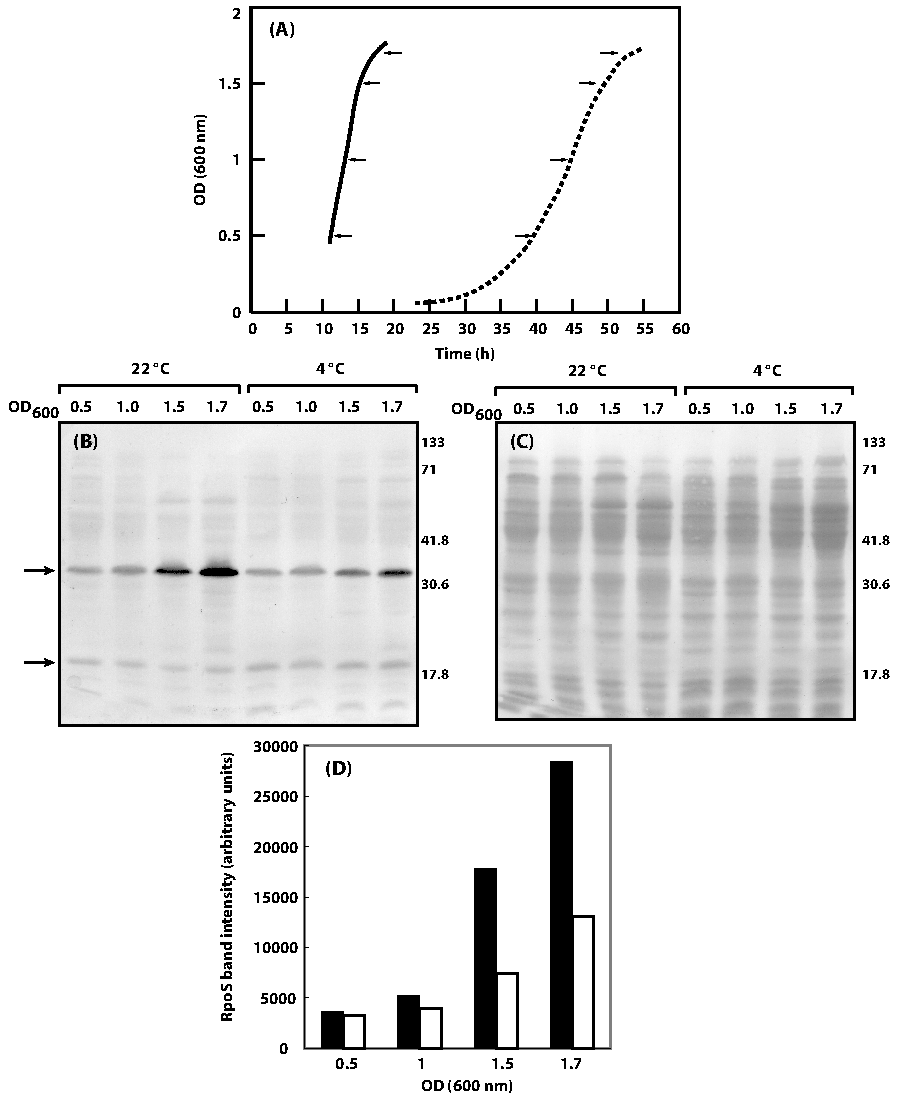
\includegraphics{figures/chap6_rpos_western_points_removed}
\end{narrow}
\caption[Growth-temperature dependant RpoS
expression]{Growth-temperature dependant RpoS expression.
\textbf{(A)} A representative growth curve of Lz4W at 22\dg{}
(solid line) and at 4\dg{} (dotted line). The growth stages of
sample collection for immunoblotting are indicated by arrows.
\textbf{(B)} Semi-quantitative immunoblot showing RpoS expression
along the growth stages in two different temperatures. The
temperatures and the OD\sub{600} for each samples are indicated on
top. Molecular weight markers in kDa are indicated on right. The
two prominent RpoS bands are indicated by arrows on left.
\textbf{(C)} Ponceau S stained blot indicating equal loading of
each samples. \textbf{(D)} Densities of the RpoS
(\U{$\sim$31}{kDa}) bands in arbitrary units measured by image
analysis. Filled bars ($\blacksquare$) and open bars ($\square$)
represent samples from cells grown at 22\dg{} and 4\dg{},
respectively.} \label{chap6_rpos_western}
\end{figure}

There was a characteristic increase in the RpoS protein level
along the grow\-th phases in Lz4W cells, both when grown at
22\dg{} (first four lanes from left to right in
Figure~\ref{chap6_rpos_western}B) and at 4\dg{} (last four lanes
from left to right in Figure~\ref{chap6_rpos_western}B).
Expectedly, RpoS level increased during entry into
stationary-phase. The increase was eight folds in cells grown at
22\dg{} (filled bars in Figure~\ref{chap6_rpos_western}D), but
only four folds when grown at 4\dg{} (open bars in
Figure~\ref{chap6_rpos_western}D). When RpoS levels at 22\dg{} and
4\dg{} were compared, it was found that the level of RpoS was less
than 50\% in cells grown at 4\dg{} to the level found in cells
grown at 22\dg{}\@. The difference was maximum at stationary-phase
(Figure~\ref{chap6_rpos_western}D). At mid-log phase (OD\sub{600}
0.5), cells from both the temperatures had comparable levels of
RpoS but when they progressed towards stationary phase the
difference became pronounced (Figure~\ref{chap6_rpos_western}D).


\subsection{Construction of a \emph{rpoS} disruption mutant}

A disruption mutant of Lz4W \emph{rpoS} was created by homologous
recombination as described in Section~\ref{chap2_disrupt} on page
\pageref{chap2_disrupt} and depicted in
Figure~\ref{chap6_rpos_disruption}. The gene was disrupted before
the amber to generate a null-mutant.



\begin{sidewaysfigure}[tbp]
\centering
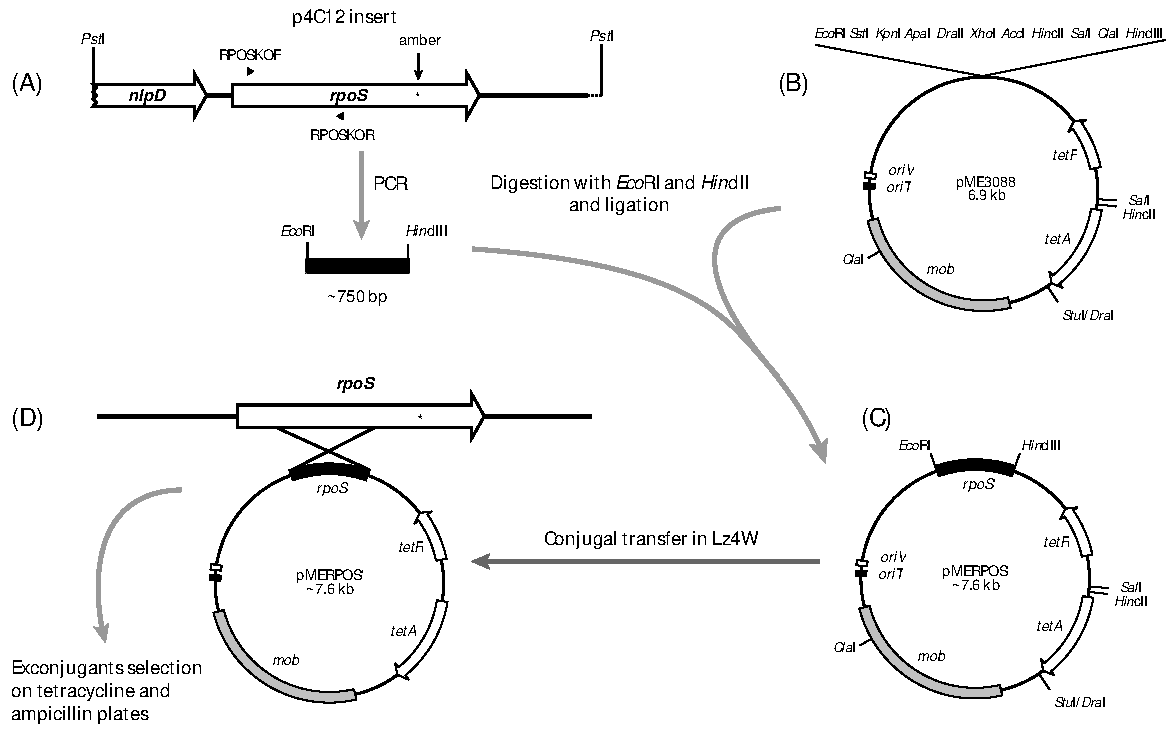
\includegraphics{figures/chap6_knock_out}
\caption[Generation of \emph{rpoS} disruption mutant]{Generation
of \emph{rpoS} disruption mutant of Lz4W. \textbf{(A)} An internal
fragment of 753 bp, before the amber mutation of the \emph{rpoS}
gene was amplified using PCR. The positions of the primers RPOSKOF
containing \emph{Eco}RI site and RPOSKOR containing \emph{Hin}dIII
site are indicated by arrow-heads\@. \emph{rpoS} and upstream
\emph{nlpD} reading frames are indicated by open arrow. The
position of the amber is shown by ``$\ast$''. \textbf{(B)} The map
of the suicide vector pME3088 with Tc\su{r} marker. \textbf{(C)}
The amplified PCR fragment was cloned into pME3088 at \emph{Eco}RI
and \emph{Hin}dIII sites. The resulting plasmid is called
pMERPOS'. \textbf{(D)} pMERPOS' was transferred into Lz4W by
conjugation. A single recombination event would knock-out
\emph{rpoS} with the integration of the whole plasmid into the
genome. The exconjugants were selected on tetracycline and
ampicillin plates. Note that the recombination event would disrupt
the reading frame before the amber.} \label{chap6_rpos_disruption}
\end{sidewaysfigure}


The strategy of \emph{rpoS} disruption relied on a single
recombination event with plasmid pMERPOS$'$ with the genomic copy
of \emph{rpoS} (Figure~\ref{chap6_rpos_disruption}D)\@. It is to
be noted that a single recombination event would result in the
integration of the whole plasmid (pMERPOS$'$) into the genome.
pMERPOS$'$ was derived from suicide vector
pME3088~\citep[Figure~\ref{chap6_rpos_disruption}B]{Schnider2000},
which lacks \emph{Pst}I site in the vector backbone. As it was
shown earlier, the insert in p4C12 detected a \U{$\sim$2.1}{kb}
\emph{rpoS} band in \emph{Pst}I digested genomic DNA from Lz4W.
Whether or not the whole pMERPOS$'$ integrated into the
\emph{rpoS} gene, could, therefore, be easily verified by probing
\emph{Pst}I digested genomic DNA with insert from plasmid p4C12.
In the disrupted strains the insert from p4C12 should detect a
band of \U{$\sim$9.7}{kb} (\U{7.6}{kb} of pMERPOS$'$ plus
\U{2.1}{kb} of genomic copy of \emph{rpoS}).


\begin{figure}[tbp]
\centering
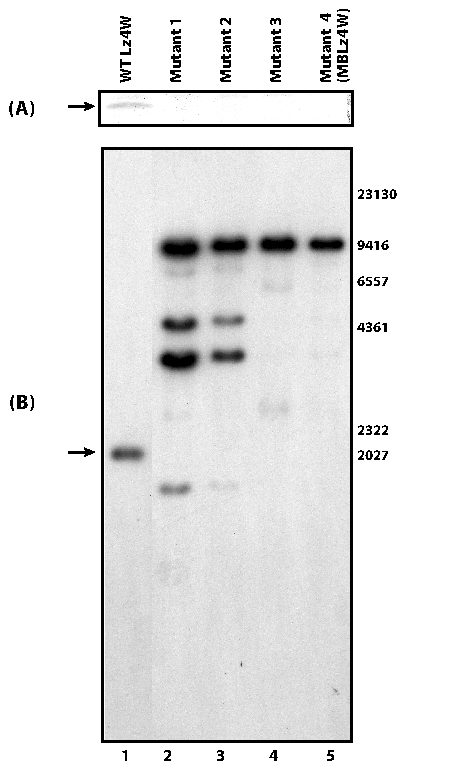
\includegraphics{figures/chap6_mutant_southern}
\caption[Construction of \e{rpoS} disruption mutant]{Construction
of Lz4W \emph{rpoS} disruption mutant. Four randomly selected
exconjugants from the disruption scheme described in
Section~\ref{chap2_disrupt} and in
Figure~\ref{chap6_rpos_disruption} was tested for the presence of
RpoS protein in immunoblot and in genomic Southern blot. The
strains used are indicated on top and the lane numbers are marked
in bottom. \textbf{(A)} Immunoblot showing the absence of the RpoS
bands in mutants (lanes 2--5). The RpoS band in the wild type (WT)
Lz4W (lane 1) is marked with an arrow. \textbf{(B)} Southern blot
analysis using \emph{Pst}I-digested genomic DNA isolated from the
mutants (lanes 2--5) and wild type Lz4W (lane 1), probed with
insert of plasmid p4C12, spanning the full-length \emph{rpoS} of
Lz4W. The \emph{rpoS} band in wild type Lz4W is marked with an
arrow. Numbers on the right show the marker positions in
base-pairs. Note the single insertion in MBLz4W.}
\label{chap6:mutant_southern}
\end{figure}

In order to verify this, the genomic DNA, isolated from four
putative mutants were digested with \emph{Pst}I and probed with
the insert of p4C12 (Figure~\ref{chap6:mutant_southern}B)\@. All
these four mutants (lanes 2--5 in
Figure~\ref{chap6:mutant_southern}B) displayed the expected
\U{$\sim$9.6}{kb} band, thus, confirming that pMERPOS$'$ indeed
had been integrated into the genome at \emph{rpoS} locus in these
mutants. It is to be noted that mutant 4 had only a single
insertion in the genome, represented by single band, whereas
mutants 1--3 had multiple insertions, represented by multiple
bands. The mutant 4 was named MBLz4W and  was used for all further
studies.

The inactivation of \e{rpoS} gene in the four randomly selected
null-mutants were also verified for the absence of the RpoS
protein by immunoblot analysis
(Figure~\ref{chap6:mutant_southern}A)\@. All these four clones
(lanes 2--5 in Figure~\ref{chap6:mutant_southern}A) were negative
for RpoS protein, confirming their RpoS-null phenotype.


\subsection{Lz4W \emph{rpoS} null-mutant is marginally cold-sensitive}

The ability of the \e{rpoS} null-mutant, MBLz4W to grow at 4\dg{}
was examined to verify the importance of \e{rpoS} during growth at
low temperature. On ABM agar plate, both the wild-type parent and
the null-mutant grew at 4\dg{}. The steady-state growth in liquid
broth (ABM) at low temperature, however, exhibited the difference
between them. MBLz4W grew slow compared with wild-type Lz4W
(Figure~\ref{chap6:mutant_cold_growth}). The effect was, however,
marginal. At 22\dg{} both these strains grew at the same rate
(open symbols in Figure~\ref{chap6:mutant_cold_growth}). The
initial long lag-phase, a characteristic feature of Lz4W growing
at cold (4\dg{}), was not altered in MBLz4W. The difference was at
the log phase, when MBLz4W grew slower (slope of the linear region
was $\sim$90\% to that of wild type) than the wild type Lz4W. This
suggested that the truncated RpoS in Lz4W, is functional, and
probably had the ability to fulfill its role during growth at low
temperature. RpoS level was, however, lower in cells growing at
low temperature than in cells growing at 22\dg{}\@. This apparent
paradox was addressed in subsequent experiments, as will be
described later in this Chapter.


\begin{figure}[tbp]
\begin{narrow}{-.5in}{-.5in}
\centering
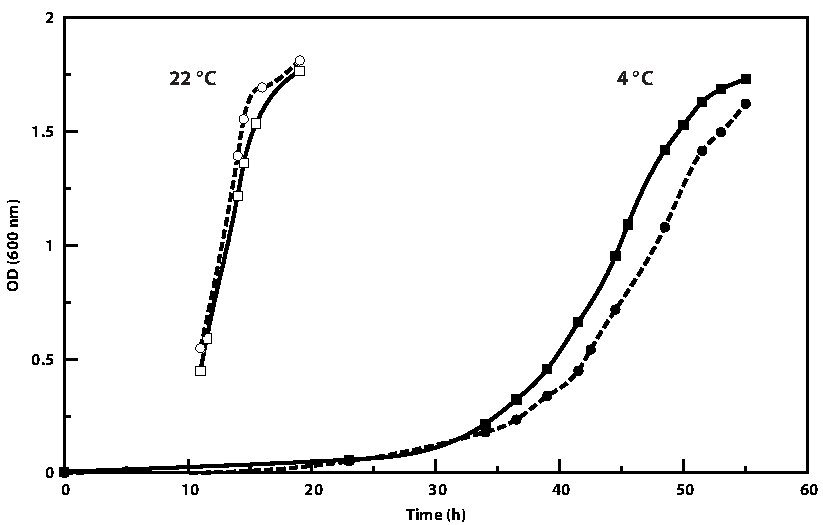
\includegraphics{figures/chap6_mutant_wild_growth}
\end{narrow}
\caption[Growth comparison between Lz4W and MBLz4W]{Growth
comparison between Lz4W and MBLz4W (\emph{rpoS}$^{-}$) in two
different temperatures. Cells grown at 22\dg{} and 4\dg{} are
indicated by open and filled symbols, respectively. Time, in hours
in X-axis is plotted against turbidity of undiluted culture,
measured as optical density (OD) at \U{600}{nm}, in Y-axis. The
data was not log-transformed, but shown raw, to emphasize the
prolonged lag-phase during growth at 4\dg{}\@. Lz4W grown at
22\dg{}, $\square$; Lz4w grown at 4\dg{}, $\blacksquare$; MBLz4W
grown at 22\dg{}, $\medcirc$; MBLz4W grown at 4\dg{},
$\medbullet$.} \label{chap6:mutant_cold_growth}
\end{figure}



\subsection{Growth of \emph{rpoS} mutant at low pH}

RpoS mutants are known to have pleiotropic effect. One of the
several known affected phenotypes is the ability to withstand
acid-shock. An attempt was, therefore, made to find out what other
stress-withstanding abilities, besides, the growth-retardation at
4\dg{}, was affected in MbLz4W. The growth properties of the
wild-type Lz4W and MBLz4W were compared at pH 5.5, both at 22 and
at 4\dg{} (Figure~\ref{chap6:growth_low_ph}).

\begin{figure}[tbp]
\begin{narrow}{-1.5in}{-1.5in}
\centering
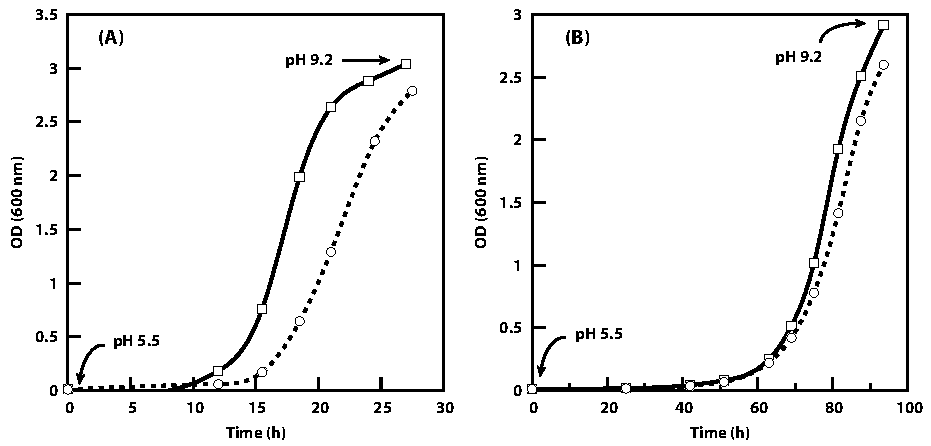
\includegraphics{figures/chap6_ph5}
\end{narrow}
\caption[Growth comparison at pH 5.5]{Growth comparison of
wild-type Lz4W ($\square$) and MbLz4W ($\medcirc$) at pH 5.5 at
22\dg{} (\textbf{A}) and 4\dg{} (\textbf{B}) in unbuffered ABM\@.
pH of the medium and the beginning (adjusted to pH 5.5) and the
end (at stationary phase, pH $\sim$9.2) of the growth are marked
with arrows. Note, the cultures become alkaline with the
progression through growth phases. The X-axis is time in hours and
the Y-axis is the turbidity of the culture, measured as optical
density (OD) at \U{600}{nm}. The culture was diluted five times
for each time point, and the measured OD, to the second decimal,
is multiplied with five, before plotting.}
\label{chap6:growth_low_ph}
\end{figure}

The steady-state growth at low pH was compared, by monitoring the
turbidity of the cultures at \U{600}{nM}. The experiments were
carried out in unbuffered rich medium (ABM), and the pH of the
medium was adjusted to 5.5 by addition of appropriate quantity of
HCl, before inoculation of the bacterial strains. It was observed
that the pH of the culture supernatant were 9.2 both for Lz4W and
MBLz4W at the completion of growth, indicating that the culture
turned alkaline during progression through growth phases.

At 22\dg{}, there was marginal increase in the duration of
lag-phase: \U{$\sim$15}{h} for MBLz4W; \U{$\sim$11}{h} for WT Lz4W
(Figure~\ref{chap6:growth_low_ph}A)\@. These values were higher
than that of the cultures growing at the same temperatures, but
under physiological pH (7.2), where as shown in
Figure~\ref{chap6:mutant_cold_growth}, both these strains reached
OD\sub{600} 0.5 at around \U{11}{h}. Apparently, growth at low pH
could prolong the lag-phase of both these strains.

In log-phase at 22\dg{}, MBLz4W grew slower than Lz4W\@. The slope
of the linear region of the curve in MBLz4W was around 68\% of the
slope observed for Lz4W (Figure~\ref{chap6:growth_low_ph}A).
MBLz4W was thus, about $\sim$30\% slow grower at pH 5.5 and at
22\dg{}\@ than Lz4W growing under same conditions.

At 4\dg{} and pH 5.5, both MBLz4W and Lz4W grew slower than the
cells grown at 4\dg{} and pH 7.0 (compare
Figure~\ref{chap6:mutant_cold_growth}B with
Figure~\ref{chap6:growth_low_ph}). While both these strains took
\U{$\sim$55}{h} to reach stationary phase when grown at pH 7.0 and
4\dg{}, they took about \U{$\sim$100}{h} to reach stationary-phase
at 4\dg{} and pH 5.5. This slow growth was evident throughout all
growth phases. However, at 4\dg{}/pH 5.5, there was no difference
in the lag-phase of growth between Lz4W and MBLz4W.

%MBLz4W, however, was marginally sensitive to simultaneous cold-
%and acid-stress, as displayed by partial growth-retardation
%(Figure~\ref{chap6:growth_low_ph}B). The difference of growth rate
% was almost identical to the difference when the same strains
%were grown at pH 7.0. At log-phase of growth, MBLz4W grew at
%around 83\% of the rate of Lz4W, as calculated from the difference
%of the slopes of the linear region of the two curves in
%Figure~\ref{chap6:growth_low_ph}B\@. Recall, MbLz4W grew at 90\%
%of the rate of Lz4W at physiological pH, at 4\dg{}\@.
%
%It can, therefore, be inferred that Lz4W is more acid-resistant
%during growth at 4\dg{} than while growing at 22\dg{}\@.
%Cold-growth associated resistance also makes these culture acid
%resistant, and this resistance is independent of \emph{rpoS}.
%MBLz4W, however, grew about two third of the rate of Lz4W at room
%temperature and at pH 5.5 in \emph{rpoS}-dependant manner. This
%further consolidates our earlier conclusion that the truncated
%$\sigma$\su{S} is indeed functional in Lz4W and in addition to its
%role in stationary-phase, it plays a important role during
%logarithmic growth of the cells.

A closure look revealed  that MBLz4W was relatively more
acid-resistant at 4\dg{} than the cells growing at 22\dg{}
(Figure~\ref{chap6:growth_low_ph}B). This ability was further
tested at extreme low pH (4.5). When MBLz4W and Lz4W were compared
for their growth capabilities at pH 4.5 and 4\dg{}, there was a
complete growth inhibition of MBLz4W (Figure~\ref{chap6:ph_4_5}).
For Lz4W, there was an extremely long lag-phase ($\sim$13 days),
but the growth rate at log-phase was not altered. The culture pH
was also became alkaline at stationary-phase. MBLz4W, on the other
hand, did not grow at all and the culture pH remained acidic.

\begin{figure}[tbp]
\centering
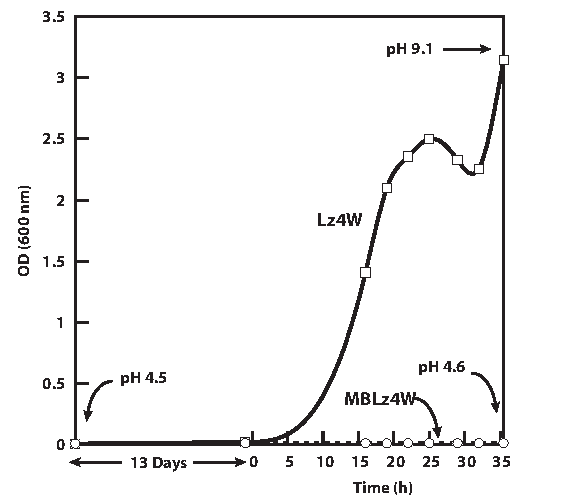
\includegraphics{figures/chap6_ph4_5}
\caption[Growth comparison at pH 4.5]{Growth comparison of Lz4W
($\square$) and MBLz4W ($\medcirc$) at pH 4.5 and 4\dg{}\@. Time
(h) in X-axis plotted against turbidity of the culture, measured
as optical density (OD) at \U{600}{nm}, in Y-axis. Note the
initial lag period of 13 days for Lz4W and the complete growth
retardation of MBLz4W. The measured pH of the culture supernatant
is indicated with arrows.} \label{chap6:ph_4_5}
\end{figure}

Putting together, the results are indicative of the role of
\emph{rpoS} during growth at extreme low pH, in cold. Furthermore,
as shown by the extremely prolonged lag-phase, the \emph{rpoS}
might play a crucial role during acclimatization of cells for
growth in such extreme conditions.

\subsection{Studies on catalase-peroxidase activity}

\emph{rpoS} is known to be involved in modulating the expression
of genes that play a role in defence against oxidative stress.
Keeping this information in mind, a detailed study on the catalase
activity Lz4W cells was carried out. Specific activities of
catalase were measured in crude extract of cell samples collected
from various phases during growth at 22\dg{} and at 4\dg{}
(Figure~\ref{chap6:catalase}A)\@. The crude cell extracts were
prepared as described in Section~\ref{crude} on
page~\pageref{crude}, and the catalase specific activity in these
extracts were measured using the method described in
Section~\ref{chap2:spec_catalase} on
page~\pageref{chap2:spec_catalase}.


\begin{figure}[tbp]
\centering
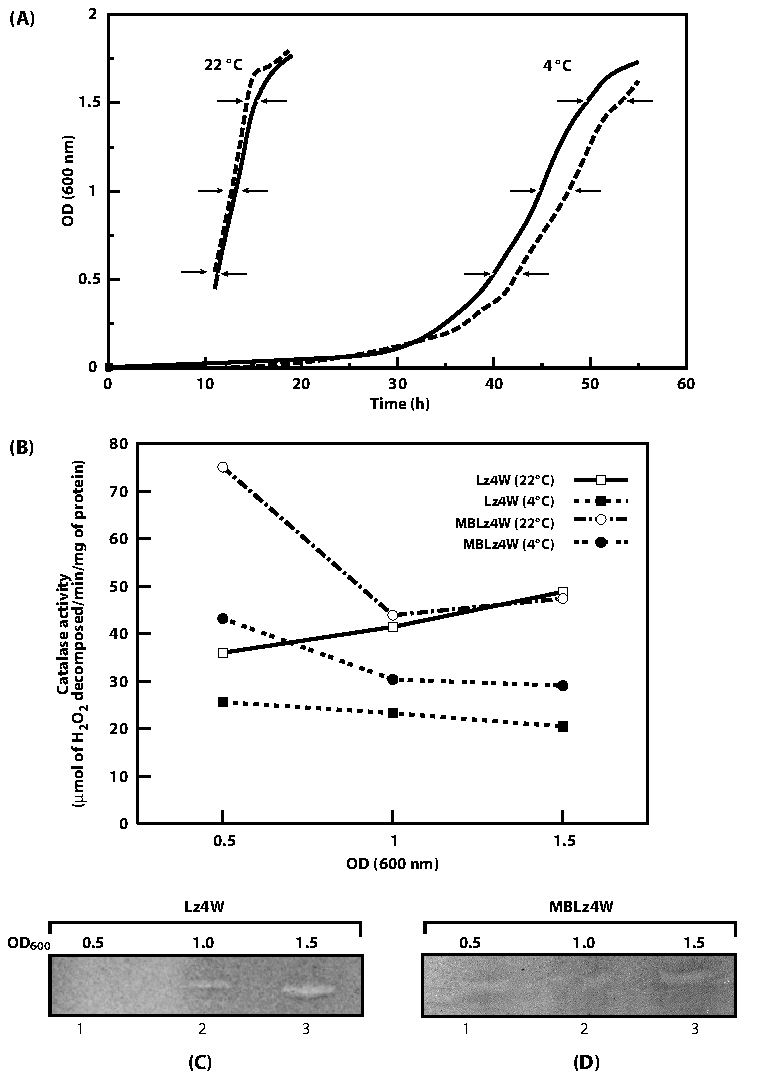
\includegraphics{figures/chap6_catalase}
\caption[Studies on catalase of Lz4W]{Studies on catalase of Lz4W.
\textbf{(A)} Growth curves of wild-type Lz4W (solid line) and
MBLz4W (dotted line) at 22\dg{} and at 4\dg{}\@. The growth phases
of sample collection are indicated by arrows. \textbf{(B)} The
catalase specific activities at 22\dg{} and 4\dg{} of samples
collected at OD\subsf{600} 0.5, 1.0, 1.5. The data plotted are the
averages of measured catalase activities of three independent
cultures. \textbf{(C)} Catalase isozyme of Lz4W detected with
activity staining in native polyacrylamide gel, in crude extract
from cells growing at 22\dg{} collected at OD\subsf{600} 0.5, 1.0,
and 1.5. The lane number indicated below and the OD\subsf{600} of
the cells are indicated on top. \textbf{(D)} Catalase isozyme of
MBLz4W detected in native polyacrylamide gel, in crude extract
from cell samples collected at OD\subsf{600} 0.5, 1.0, and 1.5.
The lane numbers and the OD of the samples are indicated as (C).}
\label{chap6:catalase}
\end{figure}

It was observed that Lz4W expresses catalase activity in growth
phase dependent manner (Figure~\ref{chap6:catalase}B)\@. During
growth at 22\dg{} ($\square$, in Figure~\ref{chap6:catalase}B) the
activity of catalase increased with the progression of the growth
phase. The activity increased from 36 units at mid-log phase
(OD\sub{600} $\sim$0.5) to $\sim$42 at late-log phase (OD\sub{600}
$\sim$1) and maximum activity was $\sim$49 at early stationary
phase (OD\sub{600} $\sim$1.5). At 4\dg{} ($\blacksquare$, in
Figure~\ref{chap6:catalase}B), however, the activity showed a
marginal decrease with the growth. The maximum activity was
observed during mid-log phase (OD\sub{600} $\sim$0.5) where the
activity was $\sim$26 units. The activity decreased with the
progression through growth phases. It was $\sim$24 and $\sim$20
units in cells at OD\sub{600} $\sim$1.0 and $\sim$1.5,
respectively.

As described in Section~\ref{chap6:rpos_expression}, during growth
at 4\dg{}, the RpoS level increases at the entry of the stationary
phase. A decrease in the catalase level at stationary phase during
growth at 4\dg{}, therefore, indicates that \emph{rpoS} is not
involved in the catalase expression in Lz4W.

In MBLz4W, however, there was an increase in the catalase
activity, both at low and high temperatures, when compared with
wild-type Lz4W (Figure~\ref{chap6:catalase}B)\@. At 22\dg{}
($\medcirc$, in Figure~\ref{chap6:catalase}B), catalase activity
was highest during mid-log phase ($\sim$75 units). The activity
decreased with progression of growth: $\sim$44 units at late-log
and $\sim$47 units at the early stationary phase. At 4\dg{}
($\medbullet$, in Figure~\ref{chap6:catalase}B), the activity,
although lower than in cells grown at 22\dg{}, was still highest
at mid-log phase, with $\sim$43 units. The activity decreased with
the progression of growth: $\sim$31 units at late-log and $\sim$30
units at early stationary phase.

The increase of catalase activity in MBLz4W was reminiscent of the
expression profile of HPI activity in \bact{Ec}, described in
\citet{Visick1997}. HPI, though earlier reported to be \emph{rpoS}
controlled~\citep{Ivanova1994}, was later shown to be upregulated
in \emph{rpoS} mutant~\citep{Visick1997}. The result reported here
for \e{P. syringae} Lz4W was, thus found to be similar to the HPI
activity in \bact{Ec}

In an effort to identify the isozymes of catalase, if any, in
Lz4W, activity staining in native polyacrylamide gel was carried
out as described in Section~\ref{chap2:activity_staining} on
page~\pageref{chap2:activity_staining}. Only one isozyme of
catalase was detected in Lz4W (Figure~\ref{chap6:catalase}C). The
band intensity increased with the progression through the growth
phases. The activity staining profile shown in
Figure~\ref{chap6:catalase} was a representative observed with
crude extract isolated from cells grown at 22\dg{}\@. The result,
therefore, corroborated the earlier measurement of specific
activity the catalase in cells grown at 22\dg{}\@. The activity
staining of the catalase in cell extract from MBLz4W
(Figure~\ref{chap6:catalase}D) also detected only one isozyme of
catalase. The expression profile in native gel, too, conformed
with the specific activity, measured earlier.

Overall, it can be inferred that there is possibly only one
isozyme of catalase present in Lz4W. Although, the expression of
this catalase at stationary phase in the room temperature grown
cells was higher than the expression detected during mid-log
phase, the increase was most probably not due to \emph{rpoS}. This
conclusion was based on the fact that during cold-growth, the
expression of catalase decreased at stationary phase, when there
was an increase in the RpoS level, measured by immunoblot
analysis. Although, the decrease was maintained in the \emph{rpoS}
null-mutant during cold-growth, the expression profile in MBLz4W
at 22\dg{} was completely opposite to the wild-type Lz4W at the
same temperature. The catalase activity was also increased in the
\emph{rpoS} mutant, indicating that a compensatory mechanism is
probably at work. This increase of activity was also highest in
the cells at mid-log phase where the activity was doubled in
mutant compared with wild-type cells.

\subsection{Construction and expression of chimeric full-length \emph{rpoS}}

As shown earlier, amber mutation in \lzsig{} results in a
truncated $\sigmaup$\su{S} (Figure~\ref{chap6_rpos_western}).
There was no indication that this amber might be suppressed by
amber-suppression or even by a read-through, as no cross reacting
band \U{>31}{kDa} was observed in immunoblot analysis.


To inquire the role of this amber mutation in \emph{rpoS}
activity, it was essential to create a full-length RpoS without
the amber, but otherwise similar in all aspects. Because, the
C-terminal half of \pasig{} from \bact{Pa} was almost identical to
the \lzsig{} and there was a suitable \emph{Bam}HI site for
cloning, it was decided that the C-terminal end of the RpoS
(\emph{BamHI}--\emph{Pst}I) on insert in plasmid p4C12 containing
\lzsig{} would be replaced with the C-terminal
(\emph{Bam}HI--\emph{Hin}dIII) fragment from plasmid pDB18R
containing, \pasig{}\@. As shown in Figure~\ref{chap6:swap}, the
exchanged region, following the \emph{Bam}HI site, would create
very little difference in the primary sequence of the protein. All
the variations in the resulting chimeric RpoS (RpoS$\chiup$)  are
summarized in Table~\ref{chap6:rpos_chi_changes}. There would be
only one non-conserved change, L298Q, in \lzsig{}. As this change
is after the amber mutation, its effect was inconsequential. There
would be only two changes before the amber, Q192H and S225T\@. As
these changes are very strongly conserved, it was presumed that
they would have little, if any, effect on the the function of
RrpoS$\chiup$ in the bacterium. \emph{rpoS}$\chiup$ would,
therefore, be very similar to \lzsig{} in all aspects, but
without the amber mutation.

\begin{sidewaysfigure}[tbp]
\centering
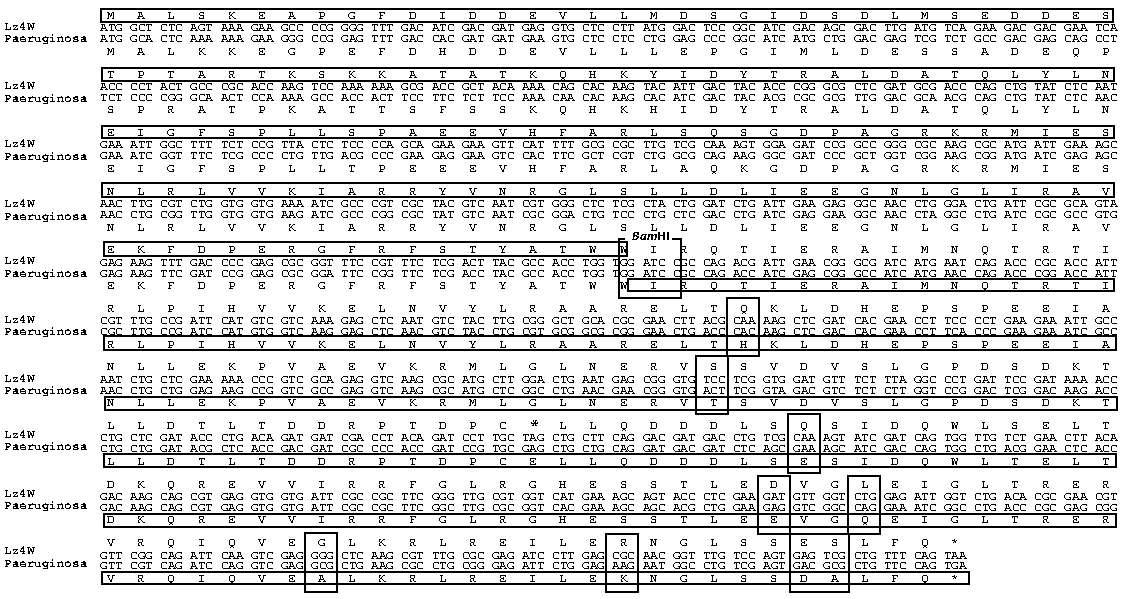
\includegraphics{figures/chap6_fusion_codon}
\caption[Domain swapping of Lz4W \emph{rpoS}]{Swapping of
C-terminal half between \emph{rpoS}\subsf{Lz4W} and
\emph{rpoS}\subsf{Pa}. The reading-frame of
\emph{rpoS}\subsf{Lz4W} and \emph{rpoS}\subsf{Pa} are aligned. The
amino acids are indicated on top of the codons for
\emph{rpoS}\subsf{Lz4W} and below codons for
\emph{rpoS}\subsf{Pa}. The amino acid sequence of the resulting
protein is indicated by the horizontal box. The \emph{Bam}HI site
(the site of exchange) is marked with a box and the amber mutation
in \emph{rpoS}\subsf{Lz4W} is marked with $\ast$. Each change of
the amino acid sequence in the resulting protein is marked with
vertical box.} \label{chap6:swap}
\end{sidewaysfigure}

\begin{table}[tbp]
\begin{minipage}[c]{\textwidth}
\renewcommand{\footnoterule}{}
\caption[Amino acid change in \emph{rpoS}$\chiup$ ]{Amino acid
changes in \emph{rpoS}$\chiup$} \label{chap6:rpos_chi_changes}
\begin{narrow}{-1in}{-1in}
\centering
\begin{small}
\begin{tabular}{p{1.5in}p{1.5in}p{1.5in}}\toprule
\textbf{Position} & \textbf{Change} & \textbf{Type of
change}\protect\footnote{Conserved and non-conserved designation
as determined by Gonnet Pam250 matrix. Strong conserved
designation denote score >0.5.}
\\\midrule\addlinespace
\multicolumn{3}{l}{\textbf{Before amber}}\\
192 & Q $\rightarrow$ H & Strongly Conserved \\
225 & S $\rightarrow$ T & Strongly Conserved \\\addlinespace
\multicolumn{3}{l}{\textbf{After amber}} \\
262 & Q $\rightarrow$ E & Strongly Conserved\\
295 & D $\rightarrow$ E & Strongly Conserved \\
298 & L $\rightarrow$ Q & Not conserved\\
314 & G $\rightarrow$ A & Conserved \\
324 & R $\rightarrow$ K & Strongly conserved\\
330 & E $\rightarrow$ D & Strongly conserved\\
331 & S $\rightarrow$ A & Strongly conserved\\
\bottomrule
\end{tabular}
\end{small}
\end{narrow}
\end{minipage}
\end{table}

The plasmid pXRPOS containing \emph{rpoS}$\chiup$ was constructed
by ligating N-terminal \emph{Pst}I--\emph{Bam}HI DNA fragment from
plasmid p4C12 containing \lzsig{} and the C-terminal
\emph{Bam}HI--\emph{Hin}dIII DNA fragment from plasmid pDB18R,
containing \pasig{}, on a broad-host-range plasmid
pGL10~\citep[Figure~\ref{chap6:pxrpos}E]{Bidle1999}. The over-all
scheme of the construction is shown in Figure~\ref{chap6:pxrpos}.
In pXRPOS, the reading frame of \emph{rpos}$\chiup$ was in the
opposite orientation to that of the \emph{lacZ} promoter of the
vector. Thus, the expression of the chimeric gene from pXRPOS, was
expected to be solely driven by the promoter of \lzsig{}.

\begin{sidewaysfigure}[tbp]
\centering
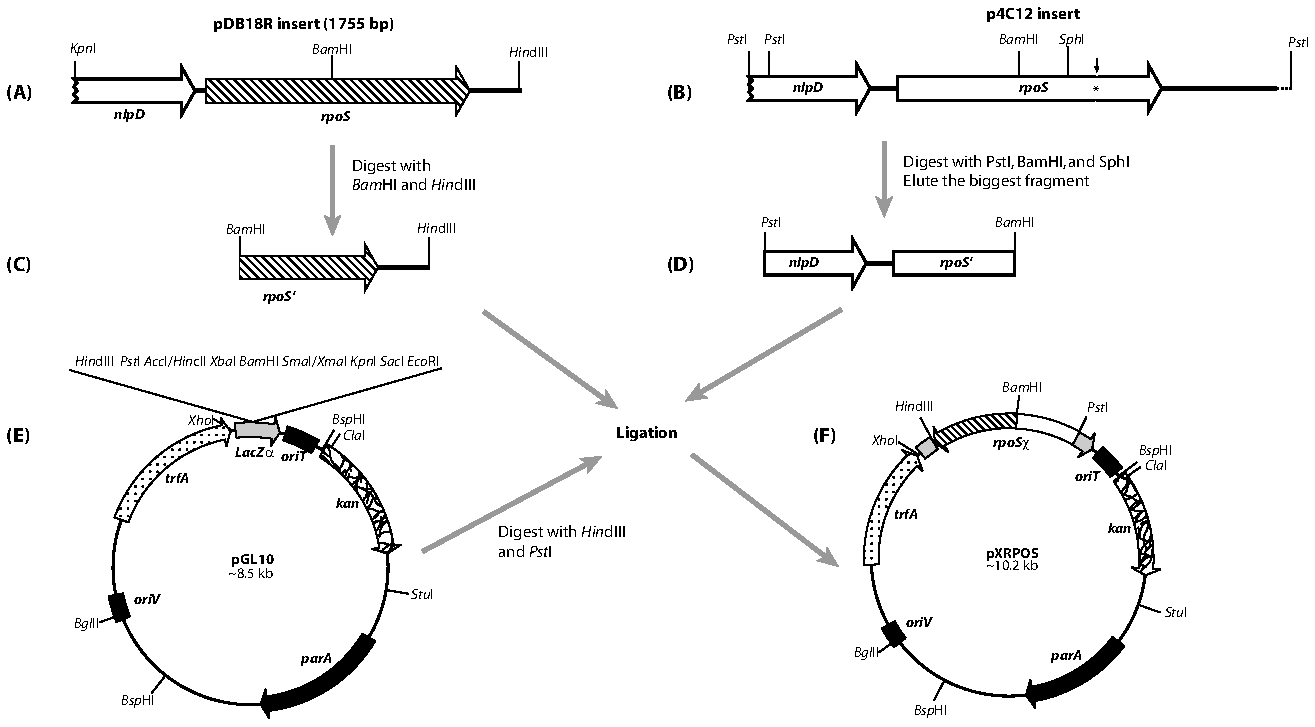
\includegraphics{figures/chap6_pxrpos}
\caption[Construction of pXRPOS]{Construction of plasmid pXRPOS,
containing chimeric, full-length \emph{rpoS}, \emph{rpoS}$\chiup$.
The C-terminal \emph{Bam}HI--\emph{Hin}dIII fragment (C) from
plasmid pDB18R (A) and N-terminal \emph{Pst}I--\emph{Bam}HI
fragment (D) from p4C12 (B) were cloned into plasmid pGL10 (E), in
a three-way ligation. The resulting plasmid, designated pXRPOS
(F), contained the chimeric \emph{rpoS} where the promoter and
N-terminal half of the gene was from Lz4W \emph{rpoS} and the
C-terminal half was derived from \bact{Pa} \emph{rpoS}. Note, in
pXRPOS, the chimeric gene was cloned in the opposite orientation
to that of \emph{LacZ} promoter of the vector.}
\label{chap6:pxrpos}
\end{sidewaysfigure}

When transformed in the null-mutant MBLz4W, pXRPOS indeed produced
a full-length RpoS protein (Figure~\ref{chap6:pxrpos_expression}).
Three independent transformed clones (lanes 1, 2, 3 in
Figure~\ref{chap6:pxrpos_expression}) were tested for the presence
of RpoS protein by immunoblot analysis. All of them exhibited the
presence of a positive band of size \U{$\sim$45}{kDa}. As it was
demonstrated earlier, MBLz4W was negative for RpoS protein on
immunoblot (Figure~\ref{chap6:mutant_southern}A), and the
cross-reacting band in Lz4W was of size \U{$\sim$31}{kDa}. RpoS in
\bact{Ec}, and \bact{Pa} is also known to migrate as
\U{41--45}{kDa} band on SDS-PAGE. It was, thus, confirmed that
\emph{rpoS}$\chiup$ on pXRPOS indeed could produce a full-length
\sigs{} in Lz4W.

\begin{figure}[tbp]
\centering
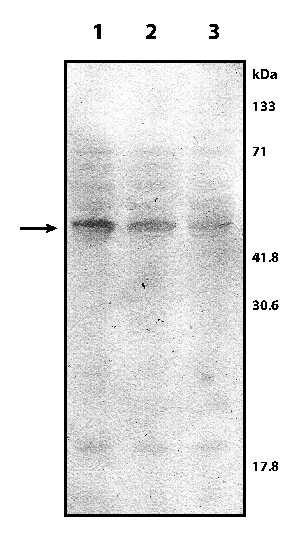
\includegraphics{figures/chap6_pxrpos_western}
\caption[Full-length \emph{rpoS} expression from
pXRPOS]{Full-length \emph{rpoS} expression from pXRPOS. Three
independent clones (lanes 1, 2 and 3) of MBLz4W, transformed with
plasmid pXRPOS was tested for the expression of RpoS in
immunoblot. Cell cultures collected at the stationary phase were
lysed directly in SDS-PAGE loading buffer and tested using
anti-RpoS antibody, as described in Section~\ref{mat:immunoblot}.
The positive band of RpoS is marked with as arrow. The molecular
weight markers are indicated on the right.}
\label{chap6:pxrpos_expression}
\end{figure}

\subsection{\emph{rpoS}$\chiup$ causes cold-sensitivity in MBLz4W}
\label{cold_sensitivity}

The effect of chimeric full-length RrpoS$\chiup$ on the growth
properties of \e{P. syringae} strains were examined in comparison
with the \lzsig{} containing the amber. Both these genes were
supplied in \emph{trans} on the same vector (pGL10). To get rid of
any effect due to the background expression of indigenous
\emph{rpoS}, the experiments were performed in MBLz4W, where the
genomic copy of the \emph{rpoS} has been disrupted. The MBLz4W was
transformed with pXRPOS, carrying the full-length chimeric
\emph{rpoS}$\chiup$, pGLSIGS, carrying the \lzsig{}. The pGLSIGS
was constructed by cloning the \emph{Pst}I insert from plasmid
p4C12 in pGL10. MBLz4W transformed with pGL10, was taken as
plasmid control.

All these strains were identical in their growth properties at
22\dg{} when grown in ABM broth (Figure~\ref{chi_growth}A).
Introduction of the plasmid, however, prolonged the time for
growth completion to \U{36}{h} from the usual \U{24}{h}.

Interestingly, at 4\dg{}, pXRPOS caused severe growth retardation
(Figure~\ref{chi_growth}B). The growth defect was prominent in
both lag-phase as well as in the log-phase. MBLz4W containing
empty plasmid vector grew fastest, while MBLz4W containing pGLSIGS
grew with an intermediate rate. MBLz4W, carrying pXRPOS took the
longest time to grow, and reached a maximum turbidity lesser than
the other two strains.

At exponential phase, MBLz4W (pXRPOS) was about 45\% slow grower,
compared with MBLz4W (pGL10), as measured by the difference of the
slope of the linear region of the growth curve shown in
Figure~\ref{chi_growth}B\@. MBLz4W (pGLSIGS) on the other hand,
was only 10\% slow grower than MBLz4W carrying pGL10.

\begin{figure}[tbp]
\begin{narrow}{-1in}{-1in}
\centering
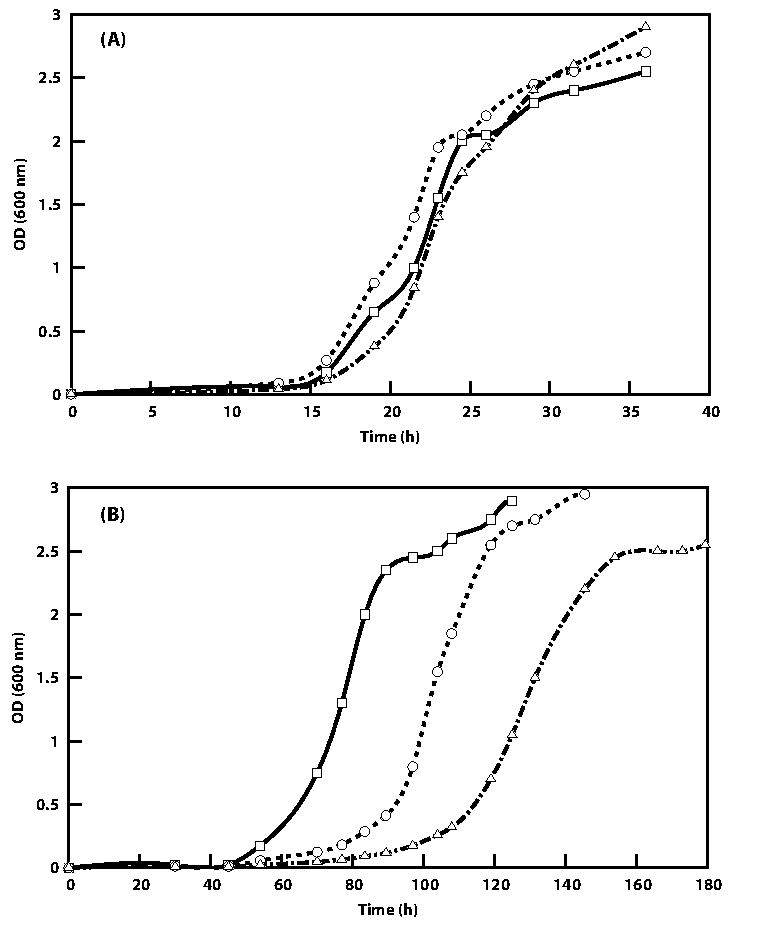
\includegraphics{figures/chap6_chimera_growth}
\end{narrow}
\caption[Growth properties of MBLz4W]{Growth comparison of MBLz4W,
transformed with pXRPOS ($\triangle$), containing chimeric
\emph{rpoS}$\chiup$, with pGLSIGS ($\medcirc$), containing
\emph{rpoS}\subsf{Lz4W}, with pGL10 ($\square$), at 22\dg{} (A)
and at 4\dg{} (B). The turbidity of the cultures measured as
optical density (OD) at \U{600}{nm} in Y-axis plotted against time
in hours at X-axis.} \label{chi_growth}
\end{figure}

Based on this result, it can be proposed that the amber, present
in the \lzsig{} reading frame, might actually confer an advantage
during exponential phase of growth at low temperature in the
wild-type Lz4W. It was shown earlier in this study, that MBLz4W
was about 10\% slow grower than the wild-type Lz4W at 4\dg{}. When
supplied in \emph{trans}, neither \lzsig{}, nor the full-length
chimeric \emph{rpoS}$\chiup$ rescued the phenotype. Instead, both
these alleles of \emph{rpoS} actually aggravated the
cold-sensitivity of MBLz4W. This can only be explained by the
assumption that the expression of plasmid borne \emph{rpoS} might
be more than the genomic copy, and this higher expression might be
responsible for the aggravated cold-sensitivity of MBLz4W. Higher
expression of RpoS is, therefore, detrimental for Lz4W during
growth at low temperature. The downregulation of RpoS expression
during cold growth, shown in Section~\ref{chap6:rpos_expression},
further supports this hypothesis.

\subsection{pXRPOS increases viability of Lz4W at stationary phase}

As shown earlier, the expression of a full-length \emph{rpoS} in
\emph{trans} caused growth retardation at 4\dg{}. In an attempt to
find whether the chimeric full-length \emph{rpoS} has any effect
other than the growth retardation at low temperature, the
survivability of MBLz4W carrying pXRPOS, pGLSIGS, and PGL10 were
tested at stationary phase during growth at 4\dg{}. Aliquots of
culture, after serial dilution were plated every \U{24}{h},
beginning with the \U{6}{h} after completion of the growth
(OD\sub{600} $\sim$3), for six days (Figure~\ref{chap6:death}).
The viability of the cells was measured as colony forming units
(CFU) per ml of the culture.

\begin{figure}[tbp]
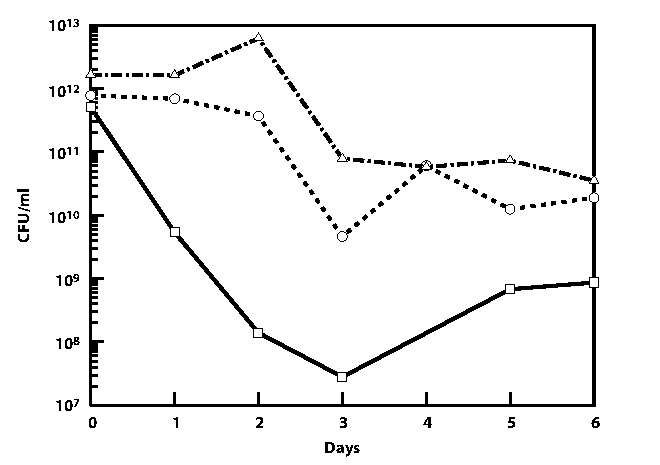
\includegraphics{figures/chap6_death}
\caption[Viability comparison of MBLz4W]{Viability of MBLz4W at
stationary phase during growth at 4\dg{}, when transformed with
pXRPOS ($\triangle$), pGLSIGS ($\medcirc$) and pGL10 ($\square$).
Viability measured as colony forming units (CFU) per ml of culture
in Y-axis is plotted against Days in X-axis. Note the
post-stationary steep viability-loss upto three days.}
\label{chap6:death}
\end{figure}

pXRPOS was found to increase  the viability of MBLz4W, compared to
the plasmid control. While there was a sharp decrease in the
viability for all the three cultures for three days after growth
completion, the viability recovered after three days. During the
initial decline, the viability dropped almost five orders of
magnitude for MBLz4W carrying the empty plasmid pGL10 ($\square$,
in Figure~\ref{chap6:death}). During that interval, the viability
loss of MBLz4W (pXRPOS) ($\triangle$) was only ten fold, and loss
was 100 fold for MBLz4W (pGLSIGS) ($\medcirc$).

After post-stationary three days, the viability recovered in all
the three strains. Interestingly, MBLz4W carrying pGLSIGS
(\e{rpoS} carrying amber) recovered to the level of the MBLz4W
carrying the full length chimeric \emph{rpoS}. At the end of the
six days, the net viability-loss for MBLz4W carrying pXRPOS and
pGLSIGS were only ten folds, while for plasmid control it was 1000
folds.

Evidently, \emph{rpoS}$\chiup$, although caused cold-sensitivity
when supplied in \emph{trans}, increased the viability of cells at
stationary phase. A noted effect of \lzsig{} was to allow the
MBLz4W cells to survive at stationary phase almost to the level of
full-length \emph{rpoS}.

\subsection{Expression level of the plasmid borne \emph{rpoS}}

As discussed in Section~\ref{cold_sensitivity}, one of the reasons
for cold sensitivity of the \emph{rpoS}$\chiup$ bearing strains
might be due to a high level of RpoS expression from the plasmid
borne \emph{rpoS}. This hypothesis was tested by directly
comparing RpoS protein levels in cells, bearing plasmid borne
\emph{rpoS}, in semi-quantitative immunoblot analysis
(Figure~\ref{chi_expression}). The RpoS protein levels were
markedly higher in cells bearing plasmid encoded RpoS, than the
strains containing only the genomic copy
(Figure~\ref{chi_expression}D)\@. Interestingly, plasmid encoded
\lzsig{} expression was lower than the plasmid encoded
\emph{rpoS}$\chiup$ (Figure~\ref{chi_expression}C), although both
were on the same plasmid (pGL10). At OD\sub{600} 0.5, the
expression of \lzsig{} was 20 folds lesser than
\emph{rpoS}$\chiup$, when supplied in \e{trans} on plasmid. With
the progression through growth phases the difference in the level
of expression decreased about 10 folds at OD\sub{600} 1.0 and
about 4 folds at OD\sub{600} 1.5.

\begin{figure}[tbp]
\begin{narrow}{-1.5in}{-1.5in}
\centering
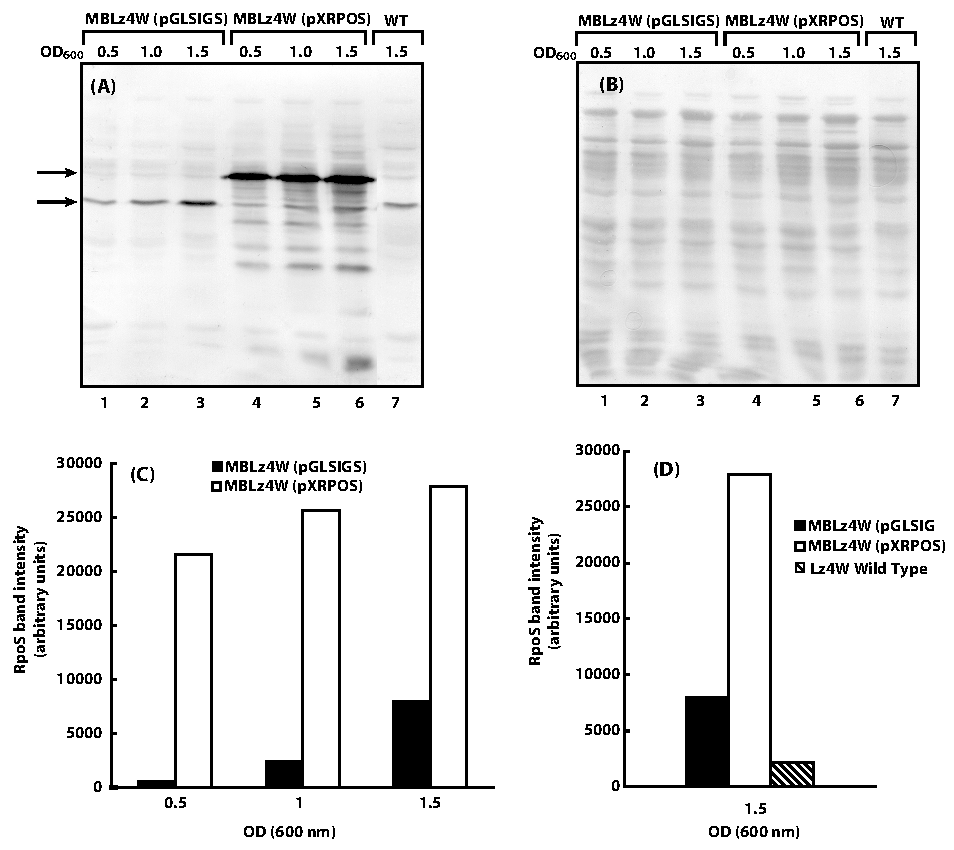
\includegraphics{figures/chap6_chi_expression}
\end{narrow}
\caption[Comparison of plasmid borne RpoS levels]{Comparison of
RpoS levels of MBLz4W, when transformed with pXRPOS, carrying
chimeric full-length \emph{rpoS}$\chiup$, pGLSIGS, carrying
\lzsig{} and the wild type Lz4W. \textbf{(A)} Immunoblot showing
the RpoS levels at 22\dg{} in cells, collected at OD\subsf{600}
0.5, 1.0 and 1.5. OD\subsf{600} of each sample is marked on top of
each lanes and the lane numbers are indicated below. The major
RpoS bands are marked with arrows. For comparison with the genomic
level of RpoS, Lz4W wild type cells of OD\subsf{600} 1.5 loaded in
lane 7. Lanes 1--3, MBLz4W, transformed with pGLSIGS; lanes 4--6,
MBLz4W, transformed with pXRPOS. \textbf{(B)} Ponceau S stained
blot showing equal loading. \textbf{(C)} Comparison of the RpoS
level between MBLz4W, transformed with pXRPOS (open bar) and
MBLz4W, transformed with pGLSIG (black bar), measured as intensity
of the RpoS band. \textbf{(D)} Comparison of the levels of RpoS
coded by genomic copy of \emph{rpoS} in wild type Lz4W (hatched
bar) with the plasmid encoded RpoS in MBLz4W, carrying
\emph{rpoS}$\chiup$ (open bar) and in MBLz4W, carrying pGLSIGS
(black bar).} \label{chi_expression}
\end{figure}


When compared with the level of expression from the genomic copy
of \emph{rpoS}, both the plasmid encoded genes showed markedly
higher expressions (Figure~\ref{chi_expression}D)\@. At
OD\sub{600} 1.5, plasmid coded \lzsig{} showed 3 folds more
expression than expression from the genomic copy. The expression
of \emph{rpoS}$\chiup$ from plasmid  was almost 12 times more than
the expression from the genomic copy. The production of RpoS was
expectedly higher when expressed from the plasmid. The unusual
high amount of RpoS produced from the plasmid encoded
\emph{rpoS}$\chiup$ is surprising. A possible explanation could be
in the difference in proteolytic degradation of the two different
types of RpoS, one being intact protein, and the other being
truncated.

\section{Discussion}

\emph{rpoS} is the master regulator of general stress response in
Gram negative bacteria~\citep{Hengge2002}. In spite of decades of
research, its exact role in each of the stress pathway remains as
elusive as ever. Only very recently, the molecular mechanisms of
regulation of \emph{rpoS} is beginning to emerge. This is not
surprising, given that the expression of \emph{rpoS} is controlled
at every possible means known to occur in cell. The knowledge of
downstream pathway of each of the stress response, however, is
still fragmentary. On one hand, the role of \emph{rpoS} in
oxidative stress response is broadly worked out, on the other hand
its role in cold-stress is, at best, arguable. Several of the
known \emph{rpoS}-controlled promoters in \bact{Ec} have been
shown to be upregulated during growth at low
temperature~\citep{Sledjeski1996,Rajkumari2001}. RpoS expression
itself is upregulated during exponential growth at low
temperature. But \bact{Ec} \emph{rpoS} mutant has no growth defect
at low temperature~\citep{Sledjeski1996}.

The work presented in this study have demonstrated that, in
contrary to findings in \bact{Ec}, Lz4W \emph{rpoS} mutant is
cold-sensitive, albeit marginally. It has also been shown that
Lz4W \emph{rpoS} harbors an amber mutation in its reading-frame,
which results in a truncated, but functionally competent protein,
as judged by the severe acid-sensitivity of the null-mutant. In
contrast to \bact{Ec}, RpoS in Lz4W is downregulated during
cold-growth. Moreover, expression of either the indigenous
\emph{rpoS} (with amber) or a full-length chimeric \emph{rpoS} in
\emph{trans} did not alleviate, rather, aggravate the
cold-sensitivity of the \e{rpoS} null-mutant.


The present study also examined the role of \emph{rpoS} during
exponential growth of Lz4W at low temperature. All the phenotypes
of the \emph{rpoS} null-mutant tested, namely growth in low pH,
low temperature, or both together showed a distinct defect at lag
and exponential growth phase, implicating a role for \emph{rpoS}
in various growth phases of this bacterium. Unfortunately, not
much is known about role of \emph{rpoS} during exponential growth,
neither in mesophiles nor in psychrotrophs. In spite of its low
expression during exponential phase~\citep{Lange1991}, \emph{rpoS}
is known to control at least two genes in \bact{Ec} during
exponential phase: \emph{xthA}~\citep{Sak1989} and
\emph{aidB}~\citep{Loewen1994}. Both these genes were shown to be
involved in repair of DNA damage in \bact{Ec}.

As shown by activity staining, there is only one catalase isozyme
present in \e{P. syringae} Lz4W\@. Although, the the expression of
this catalase is growth phase dependent, it is probably not
\emph{rpoS} dependent, because, during growth at 4\dg{}, the
catalase activity did not increase with the observed increase in
RpoS level. Moreover, the activity was higher in \e{rpoS}
null-mutant. This finding is in the line with the recent
observation that HPI level increases in \bact{Ec} \emph{rpoS}
mutant~\citep{Visick1997}. There was also earlier report that
several \siga{}-controlled gene are expressed more in \sigs{}
mutant~\citep{Farewell1998}.

If \emph{rpoS} is important during growth of the cold-adapted
\e{P. syringae} at low temperature, then why does it harbor an
amber? The answer to this question lies in the discovery of GASP
mutants (see Section~\ref{chap6:intro}). The mechanism is akin to
the selection of cancerous cells in multicellular organism and has
been explained through game theory~\citep{Vulic2001}. GASP alleles
of \emph{rpoS} are believed to be defective in density dependent
growth inhibition, and are believed to grow at the expense of the
wild type cells. One of the postulate of the theory is that GASP
mutants would have selective advantage only in presence of large
excess of wild type cells, a phenomenon described as
\emph{evolutionary cheating}. As will be discussed in the next
chapter, this theory can not explain the wide-spread mutant
alleles of \emph{rpoS} in nature, where in the absence of the wild
type cell, \emph{rpoS} GASP allele would have lost its selective
advantage. A presumptive proposition will be that the mutant
alleles of \emph{rpoS} does indeed confer a hitherto unknown
selective advantage on the cells carrying it.

The first evidence of such an advantage came from a recent work,
where it was shown that under conditions of slow growth in
chemostat culture, \emph{rpoS} mutants could be selected over wild
type cells. Moreover, under condition of dual-stress, most often,
an amber containing \emph{rpoS} gets selected and gets fixed in
the population~\citep{Mcrobb2002}. The authors argued that
upregulation of \emph{rpoD} activity is the cause for the
selection of \emph{rpoS} mutants over the wild type allele. In
situation of dual stress, an attenuated version of \emph{rpoS}
gets selected to deal with the additional stress.

Lowering of one $\sigmaup$ factor does upregulate the activity of
the others; what termed as $\sigmaup$ factor competetion
model~\citep{Farewell1998,Zhou1992}. The phenomenon is based on
the fact that in \bact{Ec}, and probably in other bacteria, the
total number of $\sigmaup$ factors ({$\sim$1200} molecules) is
more than the total number (600--700 molecules) of core enzyme
molecule available to form holoenzyme, at any give
time~\citep{Ishihama2000}.

An amber would be a way to downregulate the RpoS level during
vegetative growth but maintaining enough RpoS activity to cope
with additional stress. There are several ways this might be
achieved. First, a read-through of the amber might produce low but
sufficient RpoS, or second, depending on the position of the amber
a truncated protein might actually results in promoter
discrimination within \emph{rpoS} regulon. An indication of this
was presented in Chapter 5 of this study. How could promoter
discrimination within \emph{rpoS} regulon upregulate other
$\sigmaup$ factors? A potent way would be the regulation by
anti-$\sigmaup$ factors. For example, \emph{rsd}, the regulator of
$\sigmaup$\su{70} in \bact{Ec} was found to be \emph{rpoS}
controlled~\citep{Jishage1999}. A search for \emph{rsd} homolog in
sequenced genomes identified its homolog in all known sequenced
genomes (data not shown). In \bact{Pa}, \emph{algQ} is a potential
anti $\sigmaup$\su{70}. Lastly, a truncated $\sigmaup$ might
possess an altered binding affinity to core RNA polymerase,
thereby, modulating the level of holo RNA polymerase.

In Lz4W, the growth at exponential phase probably involves
vegetative $\sigmaup$ factor. A lowering of the \emph{rpoS} level
would potentially upregulate \emph{rpoD} activity, thereby,
promoting growth. A distinct downregulation of RpoS level was
observed during growth of Lz4W at low temperature, indicating, any
mechanism that might downregulate RpoS could potentially promote
growth at low temperature. It is also to be noted that disruption
of the \emph{rpoS} made Lz4W cold-sensitive, indicating a complete
loss of RpoS function is detrimental for growth at low
temperature. Moreover, expression of \emph{rpoS} in high level
actually made Lz4W severely cold-sensitive. Putting all these
observations together, it is obvious that the amber in the
\emph{rpoS} reading frame is actually an optimum condition, which
might have been selected during growth at low temperature.

Can this phenomenon be extended to other bacteria. There are
contradictory evidences in studies in \bact{Ec}. \emph{rpoS} is
actually upregulated in \bact{Ec} during growth at low
temperature~\citep{Sledjeski1996}. Exogenous expression of ppGpp,
the alarmone, which increases the affinity of the core RNA
polymerase to \sigs{}~\citep{Jishage2002}, makes \bact{Ec}
cold-sensitive~\citep{Jones1992}. More studies are, therefore,
required before the conclusion from the present study can be
extended to other bacteria, in more general sense.\ding{45}
